\section{Background}
\label{sec:dda:back}

\subsection{Today's Suboptimal Initial Bitrate Selection}

A video player should ideally pick the highest initial bitrate
that is sustainable (i.e., below the throughput), in order to ensure desired user experience of video
streaming. Existing approaches to initial bitrate selection, however, are
inefficient. Table~\ref{tab:video} shows measured anecdotal evidence of such
inefficiencies from several commercial providers.  Fixed-bitrate players that
use the same bitrate for the whole video session often intentionally use low
bitrate to prevent mid-stream rebuffering (e.g., NFL, Lynda). Even if bitrate
can be adapted midstream (e.g.,~\cite{dash,netflix,festive}) the player often
conservatively starts with a low bitrate and takes a significant time to reach
the optimal bitrate (e.g., Netflix).  Furthermore, for short video clips such
adaptation may not reach the desired bitrate before the video finishes (e.g., Vevo music clips).

\begin{table}[t!]
%\begin{footnotesize}
    \begin{tabular}{p{3cm}|p{3.cm}|p{3.2cm}|p{4.cm}}
    {\bf Streaming protocol}   & {\bf Examples} & {\bf Limitations} & {\bf How throughput prediction helps} \\ \hline\hline
    Fixed bitrate & NFL,Lynda, NYTimes        & Too low bitrate, a few chunks are & Higher bitrate with no re-buffering or \\ \cline{1-2}
    Adaptive bitrate & ESPN,Vevo, Netflix      &  wasted to probe throughput & long startup time
    \end{tabular}
%\end{footnotesize}
\caption{Limitations of today's video players and how they benefit from throughput prediction.
www.lynda.com  uses fixed bitrate of 520Kbps (360p) by default.  Netflix (www.netflix.com/WiMovie/70136810?tr kid=439131) takes roughly 25 seconds to adapt from the initial bitrate (560Kbps) to the highest sustainable bitrate (3Mbps).}
\label{tab:video}
\end{table}

\subsection{Dataset}
\label{subsec:dataset}

We use two datasets of HTTP throughput measurement to evaluate \name's performance: (i) a primary dataset collected by FCC's Measuring Broadband American Platform~\cite{fcc-2014} in September 2013, and (ii) a supplementary dataset collected by a major VoD provider in China. 

\begin{figure}[t!]
\centering
%\vspace{-0.4cm}
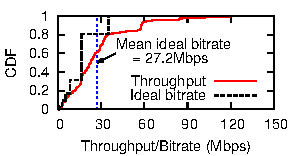
\includegraphics[width=0.5\textwidth]{figures/dda-cdf-throughput-fcc.pdf}
\caption{Distribution of throughput in the FCC dataset}
\label{fig:cdf-throughput}
\end{figure}

\mypara{FCC dataset} This dataset consists of 9.9 million sessions and is collected from 6204 clients in US spanning 17 ISPs. In each test, a client set up an HTTP connection with one of the web servers for a fixed duration of 30 seconds and attempted to download as much of the payload as possible. It also recorded average throughput at 5 second intervals during the test. 
The test used three concurrent TCP connections to ensure the line was saturated. 
%Each connection used in the test counted the numbers of bytes transferred and was sampled periodically by a controlling thread. The sum of these counters divided by the time elapsed was taken as the total throughput of the line.
%\footnote{Factors such as TCP slow start and congestion were taken into account by repeatedly transferring small chunks (256 kB) of the target payload before the real testing began. This ``warm up'' period was said to have been completed when three consecutive chunks were transferred at within 10\% of the speed of one another. All three connections were required to have completed the warm up period before the timed testing began. The ``warm-up'' period was excluded from the measurement results.}
Reader may refer to~\cite{fcc-methodology} for more details on the methodology. 

Figure~\ref{fig:cdf-throughput} shows the throughput distribution of all sessions. It also shows the distribution of ideal bitrate (i.e., highest bitrate chosen from \{0.016, 0.4, 1.0, 2.5, 5.0, 8.0, 16.0, 35.0\}Mbps\footnote{The bitrates are recommended upload encoding by YouTube~\cite{youtube-bitrates}.} below the throughput). With perfect throughput prediction, we should be able to achieve average bitrate of 26.9Mbps with no session suffering from re-buffering. Compared to the fixed initial bitrate (e.g., 2.5Mbps) used today, this suggests a large room of improvement.


The clients
%\footnote{In the FCC dataset, each client has a fixed ISP, State and Technology.} 
represent a wide spatial coverage of ISPs, geo-locations, and connection technology (see Table~\ref{tab:fcc-stats}). Although the number of targets are relatively small, the setting is very close to what real-world application providers face -- the clients are widely distributed while the servers are relatively fewer. 
%While the spatial coverage of FCC dataset naturally imitates a real-world dataset collected by a video provider, 
In addition, its measurement frequency (i.e., each client fetching content from each server once every hour) provides a unique opportunity to test the prediction algorithms' sensitivity to different measurement frequency. 
For instance, to emulate the effect of reduced data, we take one (the first) 5-second throughput sample from each test, and then randomly drop (e.g., 90\% of) the available measurements to simulate a dataset where each client accesses a server less frequently (e.g., in average once every 10 hours).

%To make it realistic, we first take one (the first) 5-second throughput sample from each test, and then we randomly drop (say, 90\%) of the history measurement of each client to simulate a dataset where each client access a server, say, in average every 10 hours. Such random dropping allows us to evaluate the prediction algorithms' sensitivity against measurement frequency, where a more robust prediction algorithm should be impacted less significantly by a higher drop rate than other algorithms.

%Besides client-side coverage, the two applications (web downloading and video streaming) represent two different types of traffic: small burst traffic (in average \fillme bytes) and long traffic (in average \fillme bytes). In \Section\ref{sec:eval}, we will discuss the different performance of various algorithms on the two applications.

\begin{table}[t]
%\begin{footnotesize}
    \begin{tabular}{p{2.2cm}|p{8.0cm}|p{3.2cm}}
 {\bf Feature} & {\bf Description}                        & {\bf \# of unique values} \\ \hline\hline
    ClientID   & Unique ID associated to a client         & 6204                \\
    ISP        & ISP of client (e.g., AT\&T)              & 17                  \\
    State      & The US state where the client is located & 52                  \\
    Technology & The connection technology (e.g., DSL)   & 5                   \\
    Target     & The server-side identification     & 30 \\
    Downlink   & Advertised download speed of the last connection (e.g., 15MB/s) & 36 \\
    Uplink     & Advertised upload speed of the last connection  (e.g., 5MB/s)   & 25 \\
    \end{tabular}
%\end{footnotesize}
\caption{Basic statistics of the FCC dataset.}
%\vspace{-0.2cm}
\label{tab:fcc-stats}
\end{table}


\myparatight{Supplementary VoD dataset} As a supplementary dataset, we use throughput dataset of 0.8 millions VoD sessions, collected by a major video content provider in China. Each video session has the average throughput and a set of features, that are different from the FCC dataset, including content name, user geolocation, user ID and server IP. This provides an opportunity to test the sensitivity of the algorithms to different sets of available features. %However, the video dataset lacks some key features, which results in lower prediction accuracy (\Section\ref{sec:eval}); for instance, the dataset only has two days and no last-connection information, so we have no access to longitudinal features (e.g., time-of-day) or connectivity features (e.g., WiFi or cable)\footnote{Note that such features are available in general (e.g., in~\cite{imc-akamai,conext13shedding})}. 
%We will focus on FCC dataset and use the VoD dataset as a supplementary dataset.


%Fortunately, this problem can be easily fixed by a {\em random dropping scheme} -- we randomly drop part (say, 90\%) of the history measurement of each client when using the dataset to predict future throughput.
%Moreover, such intense measurements also provide a nature baseline to compare the prediction accuracy with -- given a session under prediction, we can simply use the throughput of the same client and target measured in the last hour as a baseline. This baseline represents the prediction accuracy of a reasonable active measurement approach.
%In \Section\ref{sec:eval}, we will use this random dropping scheme to evaluate the accuracy of the proposed prediction algorithm.


%\begin{itemize}
%\item ClientID\footnote{In this dataset (FCC dataset), each client has a fixed ISP, State and Technology.}: Unique ID associated to a client. There are 3441 unique values.
%\item ISP: The ISP in which the client of a session is located.  There are 17 unique values.
%\item State: The US state in which the client of a session is located. There are 56 unique values.
%\item Technology: The connection technoloty (e.g., DSL, cable). There are 7 unique values.
%\item Target: The server-side identification. For WebGet, this is the target URL (10 unique values). For Video, this is the video object (78 unique values); For ping and UDP, this is the hostname of the other machine (78 unique values for ping and 75 unique values for UDP).\footnote{In each application, each client periodically sets up sessions with same Target (for instance, in the case of WebGet, each client uses wget to get the content of Target once every hour).}
%\end{itemize}

\subsection{Limitations of Simple Predictors}

This section starts by showing that simple predictors fail to yield desirable prediction accuracy, and then shows fundamental challenges of cross-session throughput prediction. 

\begin{packeditemize}
\item First, we consider the {\bf last-mile predictor}, which uses sessions with the same $\mathit{downlink}$ feature (see definition in Table~\ref{tab:fcc-stats}) to predict a new session's throughput.  This is consistent to the conventional belief that last-mile connection is usually the bottleneck. However, Figure~\ref{fig:last-mile-1} and \ref{fig:last-mile-2} show substantial prediction error\footnote{Given throughput prediction $p$ and actual throughput $q$, we define four types of prediction error: non-normalized absolute prediction error: $|p-q|$, normalized absolute prediction error: $\frac{|p-q|}{q}$, non-normalized signed prediction error: $p-q$, normalized signed prediction error: $\frac{p-q}{q}$.}, especially on the tail where at least 20\% of sessions have more than 20\% error (Figure~\ref{fig:last-mile-2}). To put it into perspective, if a player chooses bitrate based on throughput prediction that is 20\% higher or lower than the actual, the video session will experience mid-stream re-buffering or under-utilize the connection. Finally, Figure~\ref{fig:last-mile-3} and \ref{fig:last-mile-4} show that the prediction error is two-sided, suggesting that simply adding or multiplying the prediction by a constant factor will not fix the high prediction error.




\begin{figure}[t!]
\centering
%\vspace{-0.5cm}
\subfloat[Non-normalized absolute]
{
        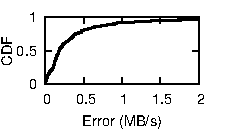
\includegraphics[width=0.25\textwidth]{figures/dda-last-mile-1.pdf}
        \label{fig:last-mile-1}
}
\subfloat[Normalized absolute]
{
        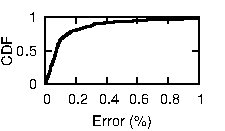
\includegraphics[width=0.25\textwidth]{figures/dda-last-mile-2.pdf}
        \label{fig:last-mile-2}
}
%\vspace{-0.5cm}
\subfloat[Non-normalized signed]
{
        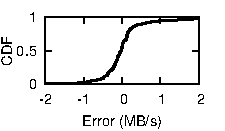
\includegraphics[width=0.25\textwidth]{figures/dda-last-mile-3.pdf}
        \label{fig:last-mile-3}
}
\subfloat[Normalized signed]
{
        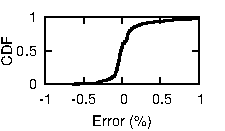
\includegraphics[width=0.25\textwidth]{figures/dda-last-mile-4.pdf}
        \label{fig:last-mile-4}
}
\caption{Prediction error of the last-mile predictor}
\label{fig:last-mile}
\end{figure}

\item Second, we consider the {\bf last-sample predictor}, which uses the throughput of the last session of the same client-target pair to predict the throughput of a future session. 
However, the last-sample predictor is not reliable as the last sample is too sparse and noisy to offer reliable and accurate prediction. 
Figure~\ref{fig:last-sample} shows that, similar to the last-mile predictor, (i) the prediction error, especially on the tail, is not desirable -- more than 25\% of sessions have more than 20\% normalized prediction error, and (ii) the prediction error is two-sided, suggesting the prediction error cannot be fixed by simply adding or multiplying the prediction with a constant factor.


\begin{figure}[t!]
\centering
\vspace{-0.5cm}
\subfloat[Non-normalized absolute]
{
        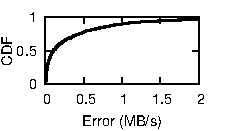
\includegraphics[width=0.25\textwidth]{figures/dda-last-sample-1.pdf}
        \label{fig:last-sample-1}
}
\subfloat[Normalized absolute]
{
        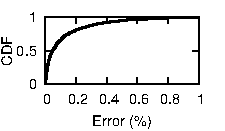
\includegraphics[width=0.25\textwidth]{figures/dda-last-sample-2.pdf}
        \label{fig:last-sample-2}
}
%\vspace{-0.5cm}
\subfloat[Non-normalized signed]
{
        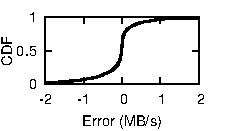
\includegraphics[width=0.25\textwidth]{figures/dda-last-sample-3.pdf}
        \label{fig:last-sample-3}
}
\subfloat[Normalized signed]
{
        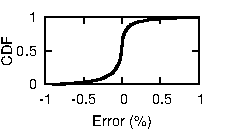
\includegraphics[width=0.25\textwidth]{figures/dda-last-sample-4.pdf}
        \label{fig:last-sample-4}
}
\caption{Prediction error of last-sample predictor}
\label{fig:last-sample}
\end{figure}

\end{packeditemize}

\begin{figure}[t!]
\centering
%\hspace{-0.5cm}
\subfloat[The average throughput of sessions matching all and a subset of three features: $\mathit{ISP=}$~Frontier, $\mathit{Technology=}$~DSL and $\mathit{Target=}$~samknows1.lax9.level3.net (X). Time: 18:00-00:00 UTC, Oct 7, 2013]
%Example of the effect of feature combinations: only sessions that are in Frontier (X), use DSL (Y) and access samknows1.lax9.level3.net (Z) have low throughput, while those sharing fewer features manifest no problem. Time: 18:00-00:00 UTC, Sep 7, 2013]
{
        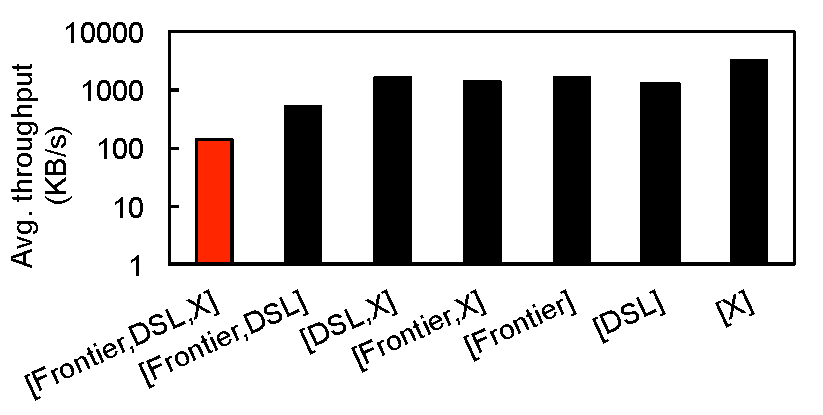
\includegraphics[width=0.45\textwidth]{figures/dda-high-dimensionality.pdf}
        \label{fig:high-dimensionality}
}
\hspace{0.5cm}
\subfloat[The relative information gain of $\mathit{Target}$ in two ISPs over time.]
%Example of same feature having different impact of different sessions: the relative information gain of the same feature (i.e., Technology) varies both across sessions in different ISPs and over time.]
{
        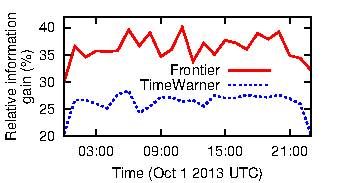
\includegraphics[width=0.45\textwidth]{figures/dda-diversity-fcc.pdf}
        \label{fig:diversity}
}
%\hspace{-0.5cm}
\caption{Two manifestations of the high complex interaction between session features and the throughput.}
\label{fig:challenges}
\end{figure}

%\tightsubsection{Challenges}
%\label{subsec:challenge}


\mypara{Challenges} The fundamental challenge to produce accurate prediction is the complex underlying interactions between session features and their throughput.
%, which make it challenging to figure out which sessions have similar throughput to the session under prediction.
In particular, there are two manifestations of such high complexity.

%The low prediction accuracy of the two simple solutions suggests a gap between what previous studies show (e.g., for each session, there are {\em some} other sessions with similar throughput) and what we need (i.e., how to identify {\em which} sessions have the similar throughput). Such gap is a result of the complex underlying interactions between session features and their throughput, which make it challenging to figure out which sessions have similar throughput to the session under prediction. In particular, there are manifestations of such high complexity.

%\mypara{High dimensionality} 
First, the simple predictors are both based on single feature (e.g., downlink or time), while combinations of multiple features often have a much greater impact on throughput than individual features. This can be intuitively explained as the throughput is often {\em simultaneously} affected by multiple factors (e.g., the last-mile connection, server load, backbone network congestion, etc), and that means sessions sharing individual features may not have similar throughput. Figure~\ref{fig:high-dimensionality} gives an example of the effect of feature combinations. It shows the average throughput of sessions of ISP Frontier using DSL fetching target samknows1.lax9.level3.net, and average throughput of sessions having same values on one or two of the three features. The average throughput when all three features are specified is at least 50\% lower than any of other cases. Thus, to capture such effect, the prediction algorithm must be expressive to combine multiple features. %Thus, algorithms such as Naive Bayes, as shown in \Section\ref{sec:eval}, could lead to low prediction accuracy.

%\mypara{High diversity} 
Second, the simple predictors both use same feature to all sessions, but the impact of same features on different sessions could be different. For instance, throughput is more sensitive to last-mile connection when it is unstable (e.g., Satellite), and it depends more to ISP during peak hours when the network tends to be the bottlenecks. Figure~\ref{fig:diversity} shows a real-world example. Relative information gain\footnote{$RIG(Y|X) = 1-H(Y|X)/H(Y)$, where $H(Y)$ and $H(Y|X)$ are the entropy of $Y$ and the average conditional
entropy of $Y$~\cite{informationgain}.} is often used to quantify how useful a feature is used for prediction. The figure shows the relative information gain of feature $\mathit{Target}$ on the throughput of sessions in two ISPs over time.
It shows that the impact of the same feature varies across sessions in different hours and in different ISPs. %It is shown that the same feature could have different impact on different sessions and over time.
%Thus, if an algorithm treats each feature (e.g., PCA which assigns a same weight to it) independently to the session under prediction, it could lead to low prediction accuracy.

We will see in Section~\ref{sec:dda:eval} that due to the complex underlying interactions between features and throughput, it is non-trivial for conventional machine learning algorithms (e.g., decision tree, naive bayes) to yield high accuracy.






